\documentclass{article}

\textwidth=6.5in
\textheight=8.5in
\voffset=-54pt
\oddsidemargin=0in
\evensidemargin=0in
\setlength{\parskip}{8pt}
\setlength{\parindent}{0pt}

\usepackage{amsmath, amssymb}
\usepackage{ifthen}

\usepackage[inline]{enumitem}
\setlist{topsep=0pt, parsep=8pt}

\usepackage[rgb,table]{xcolor}\convertcolorsUfalse
\usepackage{graphicx}

% change hyperref options
\PassOptionsToPackage{hyphens}{url}
\usepackage[bookmarks,colorlinks,linkcolor=black,citecolor=blue,pdfstartview=FitH,urlcolor=blue]{hyperref}
\hypersetup{pdfpagemode=UseNone}
\usepackage{bookmark}

\usepackage{graphicx}
\usepackage{multicol}
\usepackage{framed}
\usepackage{array}

\usepackage{icomma}

\usepackage{soul}
\usepackage[normalem]{ulem}

\usepackage{pgfplots}
\pgfplotsset{compat=1.18}  
\pgfplotscreateplotcyclelist{mycolor}{black, blue, red, green!70!black, magenta, purple, cyan, orange }  
\pgfplotsset{
  disabledatascaling,
  cycle list=tikzcolor, 
  axis lines=middle,
  every axis plot/.style={no marks, thick},
  every axis/.style={
    enlarge x limits=false,
    enlarge y limits=auto,
    xlabel style={at={(current axis.right of origin)},anchor=west},
    ylabel style={at={(current axis.above origin)},anchor=south},
    % extra x and y ticks for asymptotes
    extra x tick style={grid=major, grid style={dashed,black}},
    extra y tick style={grid=major, grid style={dashed,black}},
    /pgf/number format/1000 sep={},
  },    
  tick label style = {font=\footnotesize, fill=\currentbgcolor, inner sep=0pt},    
  xticklabel shift=1pt,    
  scaled ticks=false,
  scaled y ticks=false,
  unbounded coords=jump,
  samples=101,
  minor tick length=0,
  scatter/classes={
    open={mark=*,draw=black,fill=white, mark size=2, thin},
    closed={mark=*,draw=black,fill=black, mark size=2, thin}
  },
  width=3in,
}
\pgfplotsset{open/.style={only marks, mark=*, fill=white, thin, mark size=2}}
\pgfplotsset{closed/.style={only marks, mark=*, draw=black, fill=black,
    thin, mark size=2}}
\pgfplotsset{labeled/.style={nodes near coords, only marks, mark=*, draw=black, fill=black, thin, mark size=2, point meta=explicit symbolic}}

\pgfplotsset{gridgraph/.style={clip=false, axis line style={shorten
      >=-8pt}, xlabel style={xshift=8pt}, ylabel style={yshift=8pt},
    enlargelimits=false, grid=major, tick style={black}}} 

\usepackage{tikz}
\usetikzlibrary{
  matrix,%
  % enables the snake paths
  decorations.pathmorphing,%
  % enables bigger arrows
  decorations.markings,%
  decorations.pathreplacing,%
  decorations.text,%
  calc,%
  patterns,%
  shapes.geometric,%
  arrows,
  decorations.shapes,
  positioning,
  plotmarks,
  intersections
}
\tikzset{>=latex} % sets default arrow type in tikz
\tikzset{font=\normalsize}
\tikzset{mark size=1.5pt, mark options=thin}
\tikzset{pin distance=4pt,
  every pin edge/.style={<-, thin, shorten <= -2pt}}

\interfootnotelinepenalty=10000
\renewcommand{\thefootnote}{(\arabic{footnote})}

\usepackage{multirow, bigdelim}

% change to \usepackage[sols]{handout} to see solutions
\usepackage[]{handout}

\newcommand\iscurrentenumi[1]{%
  \ifthenelse{\equal{#1}{\theenumi}}{}{#1}}
\setenumerate[1]{ref=\#\arabic*}
\setenumerate[2]{ref=\protect\iscurrentenumi{\theenumi}(\alph*)}
\newcommand\enumiiprefix[2]{%
  \ifthenelse{{\equal{#1}{\theenumi}}\AND{\equal{#2}{(\alph{enumii})}}}{}{}%
  \ifthenelse{{\equal{#1}{\theenumi}}\AND{\NOT{\equal{#2}{(\alph{enumii})}}}}{#2}{}%
  \ifthenelse{\equal{#1}{\theenumi}}{}{#1#2}%
}
\setenumerate[3]{ref=\protect\enumiiprefix{\theenumi}{(\alph{enumii})}\roman*}

\newlength{\tipmargin}
\makeatletter

\renewenvironment{framed}{
  \setlength{\tipmargin}{\textwidth-\linewidth}
  \advance\@totalleftmargin-\tipmargin
  \def\FrameCommand{\hspace{\tipmargin}\fbox}%
  \advance\linewidth\tipmargin
  \MakeFramed {\advance\hsize-\width \FrameRestore}%
}
{\endMakeFramed}

\makeatother

\definecolor{purple}{rgb}{0.5,0,1.0}
\definecolor{hotpink}{rgb}{1, 0, 0.5}

\definecolor{skyblue}{rgb}{0, 0.5, 1}

\usepackage{fancyhdr}
\lhead{\textcolor{white}{This content is protected and may not be shared, uploaded, or distributed.}}
\rhead{}
\rfoot{\vspace*{\fill}\footnotesize\textcopyright{} \emph{Harvard Math Ma}}
\renewcommand{\headrulewidth}{0pt}
\pagestyle{fancy}
\begin{document}

\htitle{Transforming Functions}

\begin{problemonly}
  \begin{framed}

You should be able to:
    \begin{itemize}[topsep=0pt,partopsep=0pt,parsep=8pt,itemsep=0pt]
    \item Sketch $y = a f(bx) + c$, $y = a f(x + b) + c$, and $y = |f(x)|$
      from a graph of $y = f(x)$.

    \end{itemize}
  \end{framed}
\end{problemonly}

\begin{enumerate}
\item  \label{altering-functions-sqrt}

  \note{The goal of these first two parts is to recognize horizontal vs.\ vertical reflections and to think about consistency. We can find the domain and range algebraically, and these should match our graphical transformations.}

  In each part, the graph of $f(x) = \sqrt{x}$ is shown, and you're given a new function. Write a formula for the new function and sketch its graph. What are the domain and range of the new function?

  \begin{multicols}{2}
    \begin{enumerate}
    \item $a(x) = -f(x) = \fitb{1in}{- \sqrt{x}}$

      \begin{tikzpicture}
        \begin{axis}[xmin=-4.2, xmax=4.4, ymin=-4.2, ymax=4.4, width=2.9in, axis equal image]
          \addplot+[domain=0:4] {sqrt(x)};%
          \begin{solonly}
            \addplot[domain=0:4,skyblue]{-sqrt(x)};
          \end{solonly}
        \end{axis}
      \end{tikzpicture}

      Domain of $a$: $[0, \infty)$

      Range of $a$: $(-\infty, 0]$

    \item $b(x) = f(-x) = \fitb{1in}{\sqrt{-x}}$

      \begin{tikzpicture}
        \begin{axis}[xmin=-4.2, xmax=4.4, ymin=-4.2, ymax=4.4, width=2.9in, axis equal image]
          \addplot+[domain=0:4] {sqrt(x)};%
          \begin{solonly}
            \addplot[domain=-4:0,skyblue]{sqrt(-x)};
          \end{solonly}
        \end{axis}
      \end{tikzpicture}

      Domain of $b$: $(-\infty, 0]$

      Range of $b$: $[0, \infty)$

    \end{enumerate}
  \end{multicols}

  Again, you're given a new function based on $f(x) = \sqrt{x}$. If you want to graph the new function, what type of transformation should you apply to $y = \sqrt{x}$? What's one piece of information (like the domain, range, $x$-intercepts, or $y$-intercept) you could use to check which direction the transformation goes? Sketch the graph on the given axes.

  \begin{multicols}{2}
    \begin{enumerate}[start=3]
    \item

      \note{We'll probably do this together because I want to encourage students in a particular type of thinking. You do need to recognize that $f(x) + 2$ is a vertical shift of $f(x)$, but if you forget whether it's a shift up or down, is there some feature of $\sqrt{x} + 2$ that you can use? Here, thinking about the $y$-intercept or the range both work.}

      $c(x) = f(x) + 2 = \fitb{1in}{\sqrt{x} + 2}$

      \begin{tikzpicture}
        \begin{axis}[xmin=-4.2, xmax=4.4, ymin=-4.2, ymax=4.4, width=2.9in, axis equal image]
          \addplot+[domain=0:4] {sqrt(x)};%
          \begin{solonly}
            \addplot[domain=0:4,skyblue]{sqrt(x)+2};
          \end{solonly}
        \end{axis}
      \end{tikzpicture}

      Type of transformation: vertical shift

      Useful info: $y$-intercept

    \item $d(x) = f(x + 2) = \fitb{1in}{\sqrt{x + 2}}$

      \begin{tikzpicture}
        \begin{axis}[xmin=-4.2, xmax=4.4, ymin=-4.2, ymax=4.4, width=2.9in, axis equal image]
          \addplot+[domain=0:4] {sqrt(x)};%
          \solonly{\addplot+[domain=-2:4, skyblue] {sqrt(x + 2)};}%
        \end{axis}
      \end{tikzpicture}

      Type of transformation: horizontal shift

      Useful info: $x$-intercept

    \end{enumerate}
  \end{multicols}

  \pspace{\newpage}

\item 

  \note{Here, we can take advantage of the piecewise description of
    $|x|$ to say
    \[ |f(x)| =
      \begin{cases}
        f(x) & \text{ if } f(x) \geq 0 \\
        - f(x) & \text{ if } f(x) < 0 
      \end{cases}\]
    So, the parts of the graph where $f(x) \geq 0$ stay the same, and
    the parts where $f(x) < 0$ get flipped over the $x$-axis. 
  }

  \begin{problem}[0.25in]
    Here's the graph of a function $f$ with domain $[-9, 13]$. On the
    same axes, sketch $y = |f(x)|$.
  \end{problem}

  \begin{tikzpicture}
    \begin{axis}[xtick={-2.25, 3.25}, xticklabels={$-9$, $13$}, 
      xmin=-2.75, xmax=3.75, ytick=\empty, width=3in, height=2in, 
      clip=false] 
      \solonly{\addplot+[domain=-2.25:3.25, skyblue, line width=2.5pt, samples=201] {abs(-(x + 2)*(x + 1)*(x - 1)*(x -
          3))*1.1^(-x)} node[right]{$y = |f(x)|$};%
        \addplot+[closed, skyblue] coordinates { (-2.25, 6.61) (3.25, 9.21) };%
      }%
      \addplot+[domain=-2.25:3.25] {-(x + 2)*(x + 1)*(x - 1)*(x -
        3)*1.1^(-x)} node[right]{$y = f(x)$}; %
      \addplot+[closed] coordinates { (-2.25, -6.61) (3.25, -9.21) };
    \end{axis}
  \end{tikzpicture}

\item  \label{altering-1-over-x^2}

  \emph{Combining transformations.} Sketch the following, and label any asymptotes. For (b) - (e), explain how the graph is related to the graph of $y = \frac{1}{x^2}$.
  \probonly{\begin{multicols}{2} \raggedcolumns}
    \begin{enumerate}
    \item

      \note{I will have students try this on their own.}

      \begin{problem}[1.5in]
        $\displaystyle y = \frac{1}{x^2}$
      \end{problem}

      \begin{solution}
      
        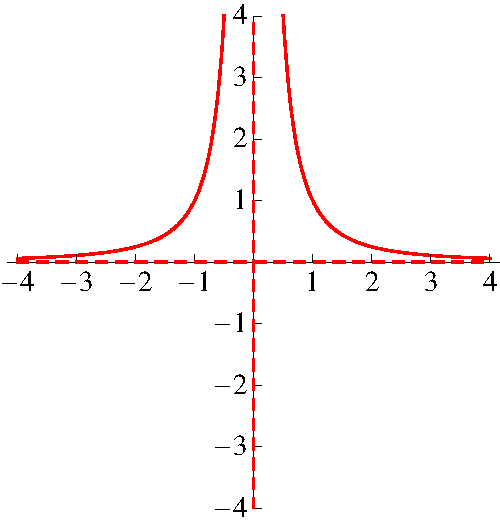
\includegraphics[width=2in]{images/altering-1-over-x^2}
        
      \end{solution}

    \item

      \note{We'll do this one together because I want to give them a bit more guidance. I'll start by asking something like: What operations do we need to do to get from $\dfrac{1}{x^2}$ to $\dfrac{3}{x^2} - 1$?}

      \begin{problem}[1.5in]
        $\displaystyle y = \frac{3}{x^2} - 1$
      \end{problem}

      \begin{solution}
        Relative to the graph of $y=\frac{1}{x^2}$, the graph is stretched in the vertical
        direction by a factor of 3, then shifted down by 1 unit.
        
        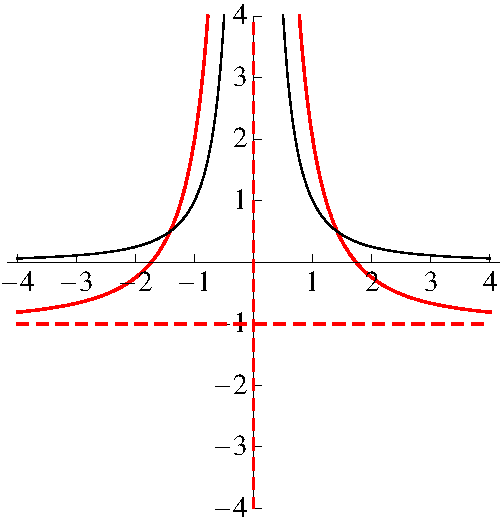
\includegraphics[width=2in]{images/altering-1-over-x^2-1}
          
      \end{solution}

    \item
      \begin{problem}[1.5in]
        $\displaystyle y = 3 \left( \frac{1}{x^2} - 1 \right)$
      \end{problem}

      \begin{solution}
        Relative to the graph of $y=\frac{1}{x^2}$, the graph is shifted down by 1 unit, then
        stretched in the vertical direction by a factor of 3.
        
        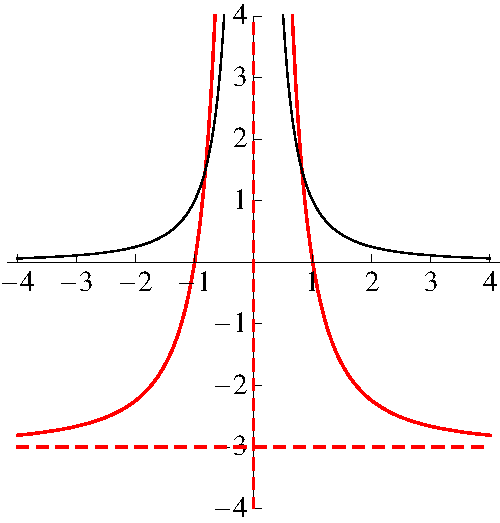
\includegraphics[width=2in]{images/altering-1-over-x^2-2}
          
      \end{solution}

    \item
      \begin{problem}[1.5in]
        $\displaystyle y = \frac{1}{(x + 4)^2} + 2$
      \end{problem}

      \begin{solution}
        Relative to the graph of $y=\frac{1}{x^2}$, the graph is shifted to the left by 4 units
        and up by 2 units.
        
        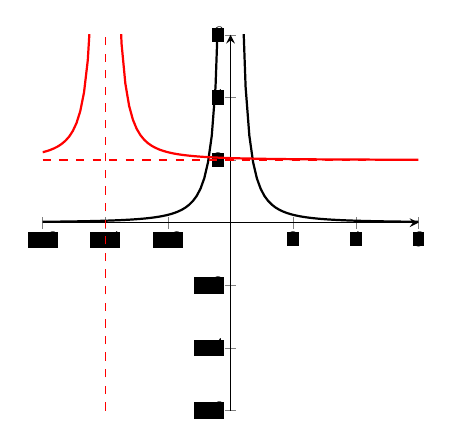
\begin{tikzpicture}
          \begin{axis}[width=2.9in, axis equal image, xmin=-6, xmax=6, ymin=-6, ymax=6,
            xtick distance=2, ytick distance=2]
            \addplot[domain=-6:6]{1/x^2};
            \addplot[domain=-6:6, red]{1/(x+4)^2 +2};
            \draw[dashed, red] (-6,2) -- (6,2);
            \draw[dashed, red] (-4,-6) -- (-4, 6);
          \end{axis}
        \end{tikzpicture} 
          
      \end{solution}

    \item
      \begin{problem}[1.5in]
        $\displaystyle y = - \frac{3}{(x - 2)^2} - 1$
      \end{problem}

      \begin{solution}
        Relative to the graph of $y=\frac{1}{x^2}$, the graph is shifted to the right by 2 units,
        stretched in the vertical direction by a factor of 3 and reflected over the $x$-axis, then
        shifted down by 1 unit.
        
        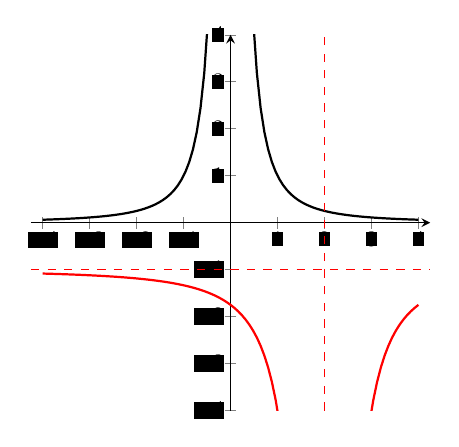
\begin{tikzpicture}
          \begin{axis}[width=2.9in, axis equal image, xmin=-4.25, xmax=4.25, ymin=-4, ymax=4,
            xtick distance=1, ytick distance=1]
            \addplot[domain=-4:4]{1/x^2};
            \addplot[domain=-4:4, red]{-3/(x-2)^2 -1};
            \draw[dashed, red] (-4.25,-1) -- (4.25,-1);
            \draw[dashed, red] (2,-4) -- (2, 4);
          \end{axis}
        \end{tikzpicture} 
          
      \end{solution}

    \end{enumerate}
  \probonly{\end{multicols}}

  \pspace{\newpage}

\item  \label{altering-functions-graph-1}

  Here's the graph of a function $f$. 

  \begin{tikzpicture}
    \begin{axis}[ytick={-1, 1}, xmin=-0.5, xmax=4.5, width=3in, height=2in]
      \addplot+[domain=0:4] {sin(90*x)}; %
      \addplot+[closed] coordinates { (0, 0) (4, 0) }; %
    \end{axis}
  \end{tikzpicture}

  \begin{enumerate}
  \item
    \begin{problem}[0.5in]
      What are the domain, range, and intercepts of $f$? (Give both the $x$- and $y$-intercepts.)
    \end{problem}

    \begin{solution}
      The domain of $f$ is $[0, 4]$, and the range of $f$ is $[-1, 1]$. The $x$-intercepts are
      $0$, $2$, and $4$, and the $y$-intercept is $0$. 
    \end{solution}

  \end{enumerate}
  In each part, you're given a function. Sketch the graph of the function, identify its domain and range, and say as much about the intercepts as you can.
  \probonly{\begin{multicols}{2}}
    \begin{enumerate}[resume]
    \item
      \begin{problem}[1.5in]
        $f(-2x)$
      \end{problem}

      \begin{solution}
          The domain of this function is $[-2,0]$, and the range is $[-1,1]$. The
          $x$-intercepts are $-2$, $-1$, and $0$, and the $y$-intercept is $0$. 

          \begin{tikzpicture}
            \begin{axis}[ytick={-1, 1}, xmin=-2.5, xmax=0.5, width=3in, height=2in]
              \addplot+[domain=-2:0] {sin(-2*90*x)}; %
              \addplot+[closed] coordinates { (-2, 0) (0, 0) }; %
            \end{axis}
          \end{tikzpicture}
      \end{solution}

    \item
      \begin{problem}[1.5in]
        $-2 f(x)$
      \end{problem}

      \begin{solution}
          The domain of this function is $[0, 4]$, and the range is $[-2,2]$. The
          $x$-intercepts are $0$, $2$, and $4$, and the $y$-intercept is $0$. 

          \begin{tikzpicture}
            \begin{axis}[ytick distance=1, xmin=-0.5, xmax=4.5, width=3in, height=2in]
              \addplot+[domain=0:4] {-2*sin(90*x)}; %
              \addplot+[closed] coordinates { (0, 0) (4, 0) }; %
            \end{axis}
          \end{tikzpicture}
      \end{solution}

    \item
      \begin{problem}[1.5in]
        $-3 f(x + 1) + 3$
      \end{problem}

      \begin{solution}
          The domain of this function is $[-1, 3]$, and the range is $[0,6]$. The
          $x$-intercept is $0$, and the $y$-intercept is $0$. 

          \begin{tikzpicture}
            \begin{axis}[ytick distance=1, xmin=-1.5, xmax=3.5, width=3in, height=2in]
              \addplot+[domain=-1:3] {-3*sin(90*(x+1))+3}; %
              \addplot+[closed] coordinates { (-1, 3) (3, 3) }; %
            \end{axis}
          \end{tikzpicture}
      \end{solution}

    \item
      \begin{problem}[1.5in]
        $3 f(2x) - 4$
      \end{problem}

      \begin{solution}
          The domain of this function is $[0, 2]$, and the range is $[-7,-1]$. There is no
          $x$-intercept, and the $y$-intercept is $-4$.

          \begin{tikzpicture}
            \begin{axis}[ytick distance=1, xmin=-0.5, xmax=2.5, width=3in, height=2in]
              \addplot+[domain=0:2] {3*sin(2*90*x)-4}; %
              \addplot+[closed] coordinates { (0, -4) (2, -4) }; %
            \end{axis}
          \end{tikzpicture}
      \end{solution}

    \end{enumerate}
  \probonly{\end{multicols}}

  \pspace{1.5in}

\item  

  \begin{problem}[0.4in]
    \emph{Revisiting the algebraic definitions of even and odd
      functions.} We've seen that a function $f$ is \uline{even} if
    $f(-x) = \fitb{0.5in}{f(x)}$ and \uline{odd} if
    $f(-x) = \fitb{0.5in}{-f(x)}$.

    Now, we can understand this in terms of graph transformations. How
    does the graph of $f(-x)$ relate to the graph of $f(x)$? Why does
    this make sense with the definitions of even and odd?
  \end{problem}

  \begin{solution}
    The graph of $y=f(-x)$ is the reflection over the vertical axis of the graph of $y=f(x)$.
    If $f$ is even, since the graph of an even function is symmetric over the vertical axis,
    the graph of $y=f(-x)$ should be the same as the graph of $y=f(x)$. 
    
    If $f$ is odd, since the
    graph of an odd function is symmetric around the origin, the graph of $y=f(-x)$ should be
    the same as the reflection over the horizontal axis of the graph of $y=f(x)$. That is,
    the graph of $y=f(-x)$ should be the same as the graph of $y=-f(x)$. 
  \end{solution}

  \pspace{\newpage}

\item  \label{understanding-horizontal-stretch}

  \note{I'm expecting students will be puzzled by why horizontal changes are ``opposite'' what you might first expect. My hope is that they will ask why this happens; if so, we'll do this problem. (I've put it at the end because I don't know when in class they might ask.)}

  Here's the graph of a function $f$ which has domain $[-3, 4]$:
  \begin{center}    
    \begin{tikzpicture}
      \begin{axis}[gridgraph, xmin=-6, xmax=8, xtick={-6, -5, ..., 10}, ytick={-10, 0, ..., 40}, ymin=-10, ymax=40, width=4in, height=2in]
        \addplot+[sharp plot] coordinates { (-3, -10) (0, 20) (2, 10) (4, 40) };
      \end{axis}
    \end{tikzpicture}
  \end{center}
  Let $g(x) = f(2x)$.

  \begin{enumerate}
  \item
    \begin{problem}[0.25in]
      Is $g(3)$ defined or undefined?
    \end{problem}

    \begin{solution}
      The output $g(3)$ corresponding to an input of $3$ is undefined, because $g(3)=f(6)$, and
      $f(6)$ is not defined. The domain of $f$ does not include $6$.
    \end{solution}

  \item
    \begin{problem}[0.5in]
      What's the domain of $g$? 
    \end{problem}

    \begin{solution}
      The domain of $g$ is $[-1.5, 2]$.
    \end{solution}

  \item

    \note{I think of what's happening here as ``$f(2x)$ pulls data from twice as far away''; in the same way, ``$f(x + 2)$ pulls data from 2 units to the right, so it ends up shifting everything left''. }

    \begin{problem}[\newpage]
      Fill in the blanks:
      \begin{alignat*}{3}
        \solonly{\textcolor{hotpink}{\bullet\ }} g(\cfitb{0.4in}{-1.5}) &= f(-3) & &= -10 \\
        \solonly{\textcolor{orange}{\bullet\ }} g(\cfitb{0.4in}{0}) &= f(0) & &= 20 \\
        \solonly{\textcolor{green!70!black}{\bullet\ }} g(\cfitb{0.4in}{1}) &= f(2) & &= 10 \\
        \solonly{\textcolor{purple}{\bullet\ }} g(\cfitb{0.4in}{2}) &= f(4) & &= 40 
      \end{alignat*}
      Use this to graph $g$ on the axes above.
    \end{problem}

    \begin{solution}
      Here are the graphs of $f$ and $g$ together, with the points colored according to the equations above.
      \begin{center}
        \begin{tikzpicture}
          \begin{axis}[gridgraph, xmin=-6, xmax=8, xtick={-6, -5, ..., 10}, ytick={-10, 0, ..., 40}, ymin=-10, ymax=40, width=4in, height=2in]
            \addplot+[sharp plot, dashed] coordinates { (-3, -10) (0, 
              20) (2, 10) (4, 40) } node[right]{$f$}; %
            \filldraw[hotpink] (-3, -10) circle(2pt); % 
            \filldraw[orange] (0, 20) circle(2pt); % 
            \filldraw[green!70!black] (2, 10) circle(2pt); % 
            \filldraw[purple] (4, 40) circle(2pt); % 
            %
            \addplot+[sharp plot] coordinates { (-1.5, -10)
              (0, 20) (1, 10) (2, 40) } node[above]{$g$}; %
            \filldraw[hotpink] (-1.5, -10) circle(2pt); % 
            \filldraw[orange] (0, 20) circle(2pt); % 
            \filldraw[green!70!black] (1, 10) circle(2pt); % 
            \filldraw[purple] (2, 40) circle(2pt); % 
          \end{axis}
        \end{tikzpicture}
      \end{center}      
    \end{solution}

  \end{enumerate}

\end{enumerate}
\end{document}
